\documentclass[UROP.tex]{subfiles}
\begin{document}

\bigskip
\section{\Large Background}
	A phased array consists of multiple antennas that can be electronically "steered" to transmit or receive a directed signal.  Phased arrays require no moving parts, and are less susceptible to mechanical failure and have significant speed advantages to traditional directional antennas.  Phased array systems are typically used in scenarios in which the antenna's beam must be rotated very quickly or the antenna must be mounted to a jostling structure that endangers the mechanical integrity of the antenna.  Phased arrays can be used for radar, communication, or imaging.   \\
	
	Phased array systems have been designed for many use cases at operating frequencies that depend on the application.  A significant amount of research and development exists for phased arrays, typically with a focus on higher frequency systems.  Higher frequencies have advantages as well serious disadvantages.  Using a high frequency allows for smaller design and faster data rates.  However, high frequency phased arrays have limited range; as the signal propagates in free space it loses power proportionally to the operating frequency.  Additionally, existing UAS's typically communicate at 900 MHz, or relatively low frequencies.
	\\
	
	This phased array system shall work at 900 MHz, which allows for communication at distances up to 20 miles with UAS's.  We propose a design that utilizes a 3D antenna array that will allow for very precise electronic steering of the signal.  \\ 
	
\begin{figure}[H]
\centering
	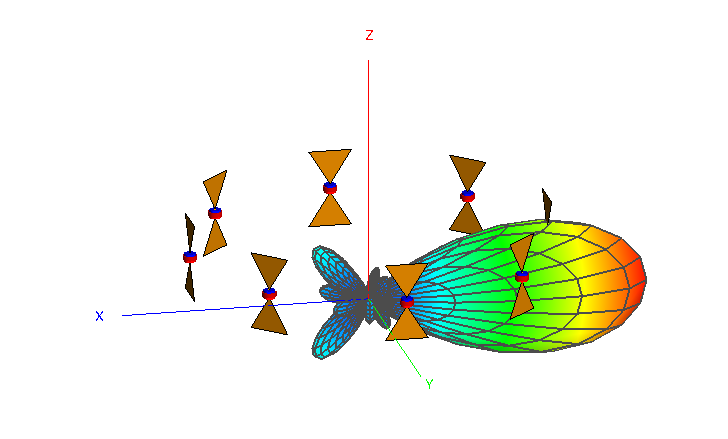
\includegraphics[scale=0.5]{PhasedArrayExample.png}
	\caption{ Phased Array example showing the ability to steer a beam\label{fig:PAexample}}
\end{figure}
	
	As seen in Fig.~\ref{fig:PAexample}, the ability to steer a beam is inherent in the design of a phased array.  By changing the delay in which the antenna elements receive the desired signal, the beam can be steered in any direction. The depicted array is a preliminary design to the 3D array that will be the final product.  
	\\
	
	Some of the students in this group worked with phased array systems and will use that experience to design a better, longer range phased array system.  Members in our group are well educated in antenna design: members have worked in RF research labs and others at RF companies. Additionally, our group will be mentored by FIRST RF and Black Swift Technologies.  Our mentors have many years of experience in the field of phased array and antenna design. 
	
\end{document}
